\chapter{Tecniche di Attacco usando la ROP e possibili mitigation}
\label{chap:Attacks}
Nei precedenti capitoli sono stati approfonditi tutti i concetti fondamentali su cui si basa la \textbf{ROP} ed il suo funzionamento. In questa parte del lavoro verranno invece spiegati differenti approcci con cui può 
essere applicata questa tecnica, in base al codice che verrà attaccato, oppure ai meccanismi di difesa attivi, o le differenti restrizioni imposte dallo sviluppatore originario del programma. Quindi, quello che 
verrà evidenziato in questi attacchi sarà la versatilità che questa tecnica offre.\\
Questa sezione avrà lo scopo di introdurre le idee che stanno alla base degli attacchi nei test. Ognuno di essi sarà poi illustrato dettagliatamente nel prossimo capitolo.\\
Inizialmente verrà riportato un classico attacco \textbf{ROP} concatenando vari \textbf{gadgets}, per poi realizzare attacchi effettuati in condizioni più scomode, ma riuscendo comunque ad applicare la tecnica.\\
In conclusione verranno introdotte alcune delle possibili tecniche di mitigazione utilizzate per fermare exploit basati sulla \textbf{Return Oriented Programming}, o più generalmente che sfruttano le vulnerabilità \textbf{buffer-overflow}.

\section{Attacco generico usando la ROP e gestendo i bad chars}
\label{sec:Attack_1}
Com'è stato ampiamente descritto nei capitoli \ref{chap:ROP} e \ref{chap:ROP-vulnerabilities}, la \textbf{Return Oriented Programming} sfrutta differenti tipi di vulnerabilità all'interno dei codici per alterare il normale 
flusso del programma. Per fare questo esso si avvale dei \textbf{gadgets}, importanti sequenze di istruzioni terminanti con una \textbf{ret}, concatenandoli assieme andando a formare una \textbf{ROP chain}.\\
Non è però sempre così scontato trovare all'interno dei binary file i gadgets necessari per costruire una \textbf{ROP chain} efficace, soprattutto se si lavora con codici relativamente brevi e poco complessi come nel caso dei 
test effettuati successivamente.\\
Nel seguente caso si è deciso di costruire una \textbf{ROP chain} che una volta inserita correttamente all'interno dello stack, fosse in grado di evocare una \textit{shell}. Tuttavia per fare questo bisognerà avvalersi di più \textbf{gadgets},
spesso non sarà direttamente possibile effettuare una particolare azione necessaria con un singolo gadget. Invece, saranno necessari più gadget in sequenza, utilizzandone di tipologie differenti e che all'apparenza 
sembrerebbero non risolvere il problema.\\ 
In questa prima fase verranno elencati alcuni dei principali \textbf{gadgets} o istruzioni che possono tornare spesso utili per la costruzione di una \textbf{ROP chain}.

\subsection*{I principali gadgets utilizzabili}
\label{par:Useful-gadgets}
Per costruire una discreta \textbf{ROP chain} diviene necessario conoscere alcune delle principali istruzioni macchina, le quali consentono di effettuare varie operazioni all'interno dei codici. Di seguito verranno elencate e spiegate quelle generalmente
più utili per effettuare un attacco \textbf{ROP} efficace con rispettive istruzioni utilizzabili \cite*{ROP-Basics}. Verrà sempre fatto riferimento al \textbf{Instruction Set} dell'architettura \textbf{x86-64} \cite*{ISA-x86-64},
e le istruzioni illustrate useranno l'\textit{Intel Syntax}, quindi verranno scritte seguendo la struttura:\\\\
\centerline{\texttt{\large{\textbf{\textcolor{Bittersweet}{COMANDO}  \space  <DESTINAZIONE>, <SORGENTE>;}}}}\\

\begin{itemize}
    \item \textbf{Caricare un dato in un registro}:\\
        Una delle azioni più utili da effettuare in una \textbf{ROP chain} è caricare dei dati all'interno dei registri. Se presente all'interno dei binary file si può utilizzare:\\
        \\\texttt{\large{\textbf{\textcolor{Bittersweet}{POP}  \space  <REG>; \space \textcolor{Bittersweet}{RET};}}}\\\\
        oppure, è possibile anche usarla concatenata ad una MOV per spostare il contenuto da un registro ad un altro. Questo, se non è disponibile una POP che carichi direttamente i dati nel registro desiderato\\
        \\\texttt{\large{\textbf{\textcolor{Bittersweet}{POP}  \space  <REG2>; \space \textcolor{Bittersweet}{MOV}  \space  <REG1>, <REG2>;}}}
    \item \textbf{Caricare in una zona di memoria un dato da un registro}:\\
        Un'altra azione che risulta particolarmente utile è caricare un dato da un registro in una zona di memoria specifica. Solitamente può essere effettuato con una MOV:\\
        \\\texttt{\large{\textbf{\textcolor{Bittersweet}{MOV}  \space  qword ptr[<REG1>], <REG2>; \space \textcolor{Bittersweet}{RET};}}}\\\\
        Il \textbf{qword ptr} significa 4 word\footnote[1]{1 word in questo caso corrisponde a 2 byte, quindi 16 bit.}, ossia 64 bit, quindi verrà caricato per intero il contenuto del registro sorgente nell'indirizzo contenuto in quello di destinazione.\\
        Se invece si vuole caricare dal registro sorgente un singolo byte nell'indirizzo contenuto in quello di destinazione (come per esempio un unico carattere), si può invece utilizzare:\\
        \\\texttt{\large{\textbf{\textcolor{Bittersweet}{MOV}  \space  byte ptr[<REG1>], <REG2>; \space \textcolor{Bittersweet}{RET};}}}\\
    \item \textbf{Caricare da una zona di memoria un dato in un registro}:\\
        Può essere utile a volte recuperare da una zona di memoria un dato per rielaborarlo all'interno di un registro, in tal caso basterà invertire le posizioni della MOV del punto precedente:\\
        \\\texttt{\large{\textbf{\textcolor{Bittersweet}{MOV}  \space  <REG1>, qword ptr[<REG2>]; \space \textcolor{Bittersweet}{RET};}}}\\
    \item \textbf{Effettuare operazioni aritmetiche con i dati nei registri}:\\
        Se necessario, è possibile effettuare operazioni aritmetiche con i dati nei registri, quali sottrazioni, addizioni, exclusive or (XOR), oppure AND. Molto spesso risulta utile mettere completamente a zero il contenuto di uno specifico registro, per farlo
        si può utilizzare:\\
        \\\texttt{\large{\textbf{\textcolor{Bittersweet}{XOR}  \space  <REG1>, <REG1>; \space \textcolor{Bittersweet}{RET};}}}\\\\
        Oppure:\\
        \\\texttt{\large{\textbf{\textcolor{Bittersweet}{AND}  \space  <REG>, 0x0; \space \textcolor{Bittersweet}{RET};}}}\\\\
        Esistono anche metodi alternativi utilizzando per esempio una MOV oppure una SUB \cite*{ZEROED-register}, tuttavia trovare le sopraccitate è molto più comune.\\
        Invece, se si necessita di sommare un valore al contenuto di un registro è possibile usare una semplice ADD:\\
        \\\texttt{\large{\textbf{\textcolor{Bittersweet}{ADD}  \space  <REG>, 0x1; \space \textcolor{Bittersweet}{RET};}}}\\\\
        Altrimenti se si vuole sommare il contenuto del registro sorgente nell'indirizzo contenuto in quello di destinazione si dovrà utilizzare:\\
        \\\texttt{\large{\textbf{\textcolor{Bittersweet}{ADD}  \space  qword ptr[<REG1>], <REG2>; \space \textcolor{Bittersweet}{RET};}}}\\
    \item \textbf{Effettuare una chiamata a sistema}:\\
        Le istruzioni che eseguono una chiamata a sistema consentono di effettuare un \textit{interrupt request} al kernel, che se gestita correttamente con i gadget precedenti darà accesso ad una \textit{shell}:\\
        \\\texttt{\large{\textbf{\textcolor{Bittersweet}{SYSCALL};}}}\\\\
        Nella precedente architettura \textbf{x86} è possibile trovare anche l'istruzione seguente per effettuare una \textbf{syscall}:\\
        \\\texttt{\large{\textbf{\textcolor{Bittersweet}{INT} \space 0x80;}}}\\\\
        Questa tipologia di istruzioni sarà molto utile soprattutto per quanto riguarda i test che verranno affrontati nel capitolo \ref{chap:Test}.\\ 
\end{itemize}

\subsection*{Esecuzione di una shell in Linux x86-64}
\label{subsec:Shell}
Dopo aver visto le principali istruzioni che possono essere utili per comporre le \textbf{ROP chain} negli attacchi, verrà approfondito quello che sarà l'obbiettivo finale dell'attacco, ossia eseguire una \textit{shell} mediante la \textbf{Return Oriented Programming}.\\
Innanzitutto, i test saranno effettuati in un sistema \textbf{Linux} sempre con architettura \textbf{x86-64}, saranno illustrati poi quali siano le convenzioni che esso utilizza per eseguire una \textit{shell}, prima di effettuare la chiamata a sistema.\\
Una chiamata a sistema effettuata con i corretti dati inseriti all'interno dei registri, consentirà di eseguire una \textit{shell}. In questa tipologia di sistema esiste tra le differenti chiamate quella a \textbf{sys\_execve} \cite*{Syscall-table}\cite*{Syscall-table-UP}, che in accordo 
alla pagina di manuale del sistema facente riferimento a tale funzione \cite*{Execve-linuxmanpage}, consente di eseguire il processo localizzato nel \textbf{pathname} memorizzato all'indirizzo di memoria passato come primo argomento della chiamata. Sarà quindi necessario impostare correttamente 
i registri del processore affinché la chiamata vada a buon fine. Seguendo quanto scritto nella \textit{System Call table} \cite*{Syscall-table} è necessario impostare i registri come segue:  
\label{shell-reg}
\begin{itemize}
    \item \textbf{rax}: 0x3b (per specificare la tipologia di chiamata, nel caso \textbf{sys\_execve});
    \item \textbf{rdi}: indirizzo in memoria della stringa ``\textbf{/bin/sh\textbackslash00}'' \space (per indicare il pathname del file da eseguire);
    \item \textbf{rsi}: 0x0 (per indicare che non verranno passati altri argomenti);
    \item \textbf{rdx}: 0x0 (per indicare che non verrà passata nessuna variabile d'ambiente\footnote[1]{Un array di stringhe che descrivono l'ambiente (environment).}).
\end{itemize}

Per comporre la \textbf{ROP chain} sarà necessario trovare i gadgets che consentano d'impostare correttamente i registri per eseguire la \textit{shell}. Inoltre, bisognerà trovare l'indirizzo di una zona di memoria in cui è consentito scrivere per poter memorizzare la stringa 
``\textbf{/bin/sh}'' da passare come argomento alla chiamata. Infine, verrà inserita come ultima istruzione della chain una \textbf{syscall}.\\
A questo punto l'attacco sarebbe completo e funzionante se non fosse che spesso all'interno dei codici esistano dei controlli per quelli che vengono comunemente definiti ``\textbf{Bad Chars}''.

\subsection*{Gestione dei Bad Chars}
\label{subsec:Badchars}
I ``\textbf{Bad Chars}'', anche chiamati ``invalid characters'', sono caratteri ricevuti e filtrati dal programma di destinazione di un attacco che fungono da delimitatori.\\
Attraverso gli algoritmi interni del programma, i \textbf{bad chars} eliminano quelli che potrebbero essere caratteri essenziali per effettuare l'attacco voluto, oppure li sostituiscono con altri valori, rendendo di fatto invano il tentativo effettuato dall'attaccante.\\
La ricerca di questi caratteri diviene conseguentemente parte cruciale dello sviluppo di un exploit, poiché, se non correttamente individuati e soprattutto evitati durante la stesura della propria \textbf{ROP chain} o payload da inviare, lo renderanno inutile. Questo perché i caratteri identificati come 
tali verrebbero mal interpretati dal sistema di destinazione, portando spesso alla terminazione del processo.\\
Quando vengono inseriti dati all'interno di un software esso ha il compito di elaborarli. Durante tale operazione, finché non raggiungeranno il punto in cui avrà effetto l'attacco, esso controlla, filtra, sostituisce oppure blocca determinati caratteri. Questo rende più complicato lo sviluppo dell'exploit. Tuttavia, esistono diversi 
metodi per identificare questi speciali caratteri e quindi evitarli nel ``payload'' finale.\\
Ad esempio, una delle possibili soluzioni per identificare questi \textbf{bad chars}, potrebbe essere analizzare il programma da quando i dati sono stati inseriti fino a quando avranno raggiunto il punto in cui avrà luogo l'exploit. Verificando se il software abbia effettuato qualche operazione su di essi.\\ 
Questo risulta essere uno dei metodi più efficaci ed allo stesso tempo uno dei più tediosi da applicare, soprattutto se il programma effettua controlli multipli e manipola più volte i dati inseriti. \cite*{Badchars}\\
Un'altra opzione, che come si vedrà è anche quella che è stata adottata durante i test, può essere quella di passare al programma una stringa contenente tutti i possibili caratteri e verificare cosa accada ad ognuno di essi durante l'esecuzione. Confrontando poi la stringa inserita con quella ottenuta una volta raggiunta la fase 
in cui avrà effetto l'attacco.\\
Una volta identificati i \textbf{bad chars} all'interno del codice, è necessario trovare un modo per evitarli. Grazie alla \textbf{Return Oriented programming}, è possibile trovare dei \textbf{gadgets} che elaborino e modifichino i dati successivamente il loro inserimento all'interno del programma eludendo i successivi controlli.
Ad esempio, se si necessita di inserire i caratteri di una specifica stringa evitando che alcuni di essi vengono considerati \textbf{bad chars} dal software, una possibilità potrebbe essere quella di inserire inizialmente una stringa con dei caratteri diversi da quelli voluti. Andando poi, mediante delle \textbf{ADD}, ad incrementare il valore 
esadecimale dei singoli caratteri, sarà possibile ottenere quelli attesi e necessari per portare a termine l'attacco.\\
Questo metodo sarà anche quello adottato durante i test, e che quindi verrà anche visto direttamente in azione.\\
Una volta gestiti correttamente i \textbf{bad chars}, se la \textbf{ROP chain} sarà stata costruita correttamente, verrà eseguita con successo una \textit{shell}.

\section{Attacco effettuando il dirottamento dello stack (stack pivoting)}
\label{sec:Attack_2}
Nella sezione precedente è stato affrontato un classico attacco \textbf{ROP} gestendo quelli che vengono comunemente definiti \textbf{bad chars} nell'ambito degli attacchi informatici.\\
Tuttavia, all'interno dei programmi accade spesso che vi siano delle limitazioni sulla lunghezza massima dell'input inseribile, oppure che nello stack non vi sia abbastanza spazio disponibile per eseguire un exploit completo.\\
Esiste una tecnica che permette di superare i problemi sopraccitati, definita \textbf{Stack Pivoting} o ``Dirottamento dello stack''. Essa prevede che l'attaccante prenda controllo del registro 
\textbf{rsp}, che, come visto nella sezione \ref{subsec:registers}, mantiene al suo interno l'indirizzo di memoria in cui risiede l'ultimo elemento dello stack frame attuale. Successivamente, tale indirizzo dovrà essere sostituito con quello di un buffer su cui in precedenza era stata scritta la \textbf{ROP chain} completa, senza alcun 
limite sulla dimensione e camuffando di fatto la posizione dello stack.\\ 
Per eseguire questa tecnica, bisognerà conoscere un indirizzo di memoria di un buffer che verrà reso successivamente il ``falso'' stack. Sarà inoltre di primaria importanza trovare dei gadgets che consentano di sostituire il valore del registro \textbf{rsp}, senza utilizzare troppo spazio dello
stack ``reale'' viste le condizioni imposte \cite*{Stack-pivoting}. Alcuni di essi verranno elencati di seguito.\\
La struttura delle istruzioni farà sempre riferimento a quella vista nella sezione \ref{par:Useful-gadgets}.
\begin{itemize}
    \item \texttt{\large{\textbf{\textcolor{Bittersweet}{POP}  \space  RSP; \space \textcolor{Bittersweet}{RET};}}}\\\\
    Questo gadget rappresenta la soluzione più semplice ed efficace, allo stesso tempo però è anche una delle meno comuni da trovare nei file. Se presente è sempre conveniente utilizzarla.
    \item \texttt{\large{\textbf{\textcolor{Bittersweet}{POP}  \space  <REG>; \space \textcolor{Bittersweet}{XCHG}  \space  <REG>, RSP; \space \textcolor{Bittersweet}{RET};}}}\\\\
    Se presente un'istruzione POP <REG> o un gadget che la contiene, è possibile concatenarla con un XCHG che coinvolga il registro della precedente POP e \textbf{rsp} per cambiarne il contenuto, occupando solamente 16 byte dopo l'indirizzo di ritorno.
    \item \texttt{\large{\textbf{\textcolor{Bittersweet}{LEAVE}; \space \textcolor{Bittersweet}{RET};}}}\\\\
    Questa rappresenta invece una delle possibilità più interessanti per dirottare lo stack e richiede solamente 8 byte dopo l'indirizzo di ritorno, quindi pochissimo spazio. Questo gadget è trovabile al termine di qualsiasi funzione (escluso \textbf{main}), ed è ciò che lo rende un'ottima alternativa a quelli illustrati in precedenza.
    Per comprenderlo a fondo è necessario capire ciò che accade durante una LEAVE, infatti anche se all'apparenza potrebbe sembrare un'istruzione poco funzionale per l'obbiettivo finale, in realtà essa è una MOV RSP, RBP seguita da una POP RBP. Questo significa che, se si ha la possibilità di sovrascrivere quello che sarà l'indirizzo
    caricato poi nel registro \textbf{rbp} durante l'esecuzione della LEAVE, inserendo successivamente tale gadget sopracitato nella \textbf{ROP chain}, il contenuto di \textbf{rsp} sarà quello voluto dall'attaccante, una volta effettuata la chiamata.
\end{itemize}
Recuperato il gadget necessario per sostituire il contenuto di \textbf{rsp}, e dopo aver correttamente inserito la \textbf{ROP chain} completa per eseguire una shell (come quella vista nella sezione \ref{subsec:Shell}) all'interno del buffer sotto il controllo dell'attaccante, sarà nuovamente eseguita con successo una \textit{shell}.

\section{Attacchi sfruttando le librerie collegate}
\label{sec:Attack_3}
Nei due attacchi visti precedentemente, l'obbiettivo era quello di sfruttare i gadgets presenti \textbf{solamente} all'interno del binary file del codice sotto attacco, per costruire un exploit usando la \textbf{Return Oriented Programming} che consentisse all'attaccante di eseguire correttamente una \textit{shell}.
Tuttavia, accade spesso che all'interno del solo binary file del codice vulnerabile, non siano presenti abbastanza gadgets per effettuare quanto richiesto dall'utente malintenzionato. Vengono allora presi in causa anche i file delle librerie collegate al programma. \cite*{Ret2libc}\\
Verranno affrontati due approcci differenti a tale situazione: 
\begin{itemize}
    \item \textbf{Prima situazione}: l'attaccante è a conoscenza della libreria collegata e dispone del suo file.
    \item \textbf{Seconda situazione}: l'attaccante non conosce la versione di libreria standard collegata al codice.  
\end{itemize}
Prima di spiegare in dettaglio le due situazioni, diviene essenziale illustrare i tre elementi fondamentali atti alla comprensione dei suddetti attacchi, ossia: la tecnica di difesa \textbf{ASLR} (\textbf{Address Space Layout Randomization}), che era stata descritta nella sezione \ref{sec:Def-bypass}, la \textbf{Procedure Linkage Table} 
(\textbf{PLT}) e la \textbf{Global Offset Table} (\textbf{GOT}).\\ L'\textbf{ASLR} sarà il principale ostacolo in questa tipologia di attacchi \cite*{ASLR-BYPASS}, essa rende complesso l'utilizzo delle procedure all'interno delle librerie condivise negli attacchi \textbf{ROP}, rendendo casuali gli indirizzi su cui esse risiedono in memoria, ogni qualvolta il programma a cui sono collegate sia eseguito.

\begin{figure}[htpb]
    \centerline{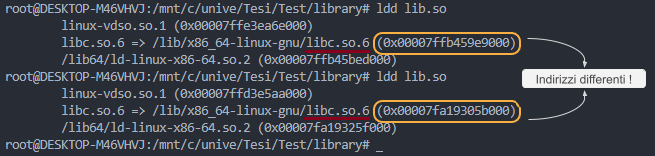
\includegraphics[scale=.8]{images/ASLR-ldd.png}}
    \caption{Esempio della randomizzazione degli indirizzi di partenza della \textbf{libc} dopo la sua esecuzione.}
    \label{fig:ASLR}
\end{figure}

Le due tabelle sopraccitate, invece, saranno il principale motivo per cui sarà possibile bypassare la meccanica di difesa appena riportata, utilizzando la \textbf{Return Oriented Programming}.\\ 
Sarà necessario andare ad approfondire quale sia il loro ruolo all'interno del processo di esecuzione di un programma, per comprendere come questo sia possibile.

\subsection*{Procedure Linkage Table (PLT) e Global Offset Table (GOT)}
\label{subsec:PLT-GOT}
In questa sezione verranno spiegati i concetti fondamentali della \textbf{Procedure Linkage Table} (\textbf{PLT}) e \textbf{Global Offset Table} (\textbf{GOT}), due importanti componenti di un qualsiasi \textbf{Executable and Linkable Format} (\textbf{ELF})\footnote[1]{l'\textbf{ELF} è un comune standard di formato per file quali \textit{eseguibili}, \textit{codice oggetto}, \textit{librerie condivise}, e \textit{core dumps}, usato anche nei sistemi Linux.} 
file negli eseguibili in Linux \cite*{ELF}\cite*{ELF2}. In particolare, queste due porzioni sono essenziali per capire come avviene il collegamento alle librerie e l'esecuzione di un programma in questo sistema, e successivamente, come potranno essere utili per eseguire gli attacchi.\\
Quando viene sviluppato un programma in linguaggio C, nella maggior parte dei casi si utilizzano delle librerie, ossia insiemi più o meno grandi di funzionalità già disponibili e testate da altri utenti. Tuttavia, per poter richiamare queste funzioni, le librerie dovranno essere prima collegate al codice 
che ne richiederà l'utilizzo. Esistono due metodi differenti con cui verrà effettuato il collegamento delle librerie alla propria applicazione: lo \textbf{Static Linking} e il \textbf{Dynamic Linking}. Quale dei due sarà utilizzato dipenderà dalla tipologia di libreria che si usufruirà.\cite*{LIBRARY}\\
Con il primo sistema il programma viene collegato ad una \textbf{libreria statica} a \underline{compile time} (tempo di compilazione), ed il codice contenuto in essa diviene parte integrante di quello dell'applicazione stessa. Mentre con il secondo, una volta inserito il nome della \textbf{libreria dinamica} (o anche \textit{shared library} in linux) nel binary file dell'applicazione, il codice \underline{non sarà copiato} in quello del proprio software come nel primo 
caso, ma sarà caricato in memoria e collegato ad esso dal sistema, una volta eseguito il programma \cite*{PLT-GOT}. Tale metodologia, essendo le funzionalità richieste dall'applicativo collocate in zone di memoria ad esso sconosciute ad ogni suo nuovo avvio, necessiterà di un modo rapido per far sì che questi indirizzi possano essere comunque sempre recuperati e forniti ad esso.\\
A tale scopo, sono state create le due sezioni sopraccitate, \textbf{PLT} e \textbf{GOT}.\\
La \textbf{Procedure Linkage Table} è una tabella di tipo \textit{read-only} ed è responsabile di richiamare il \textbf{dynamic linker} durante e dopo l'esecuzione del programma, per risolvere gli indirizzi delle funzioni da esso richieste e di cui non si conosce l'indirizzo di posizionamento in memoria \cite*{PLT-GOT-OVERWRITE}. Essa può essere trovare col nome ``\textbf{.plt}'' all'interno del file ELF dell'applicazione.\\
Invece i sistemi operativi moderni hanno ``due'' \textbf{Global Offset Table} per ogni processo, una chiamata ``\textbf{.got}'' ed un'altra ``\textbf{.got.plt}''. Per quanto riguarda questo lavoro, ci si concentrerà solamente sulla seconda, che assieme alla ``\textbf{.plt}'' si occuperanno di effettuare la risoluzione degli indirizzi delle funzioni esterne mediante una tecnica chiamata ``\textbf{Lazy Binding}''.\\
Per comprendere al meglio il ruolo delle due sezioni è più conveniente introdurre prima questa meccanica. Essa prevede che gli indirizzi assoluti delle funzioni esterne non siano risolti, finché esplicitamente chiamati per la prima volta nel codice del software. Essa venne introdotta per limitare i tempi di avviamento dei programmi e lo spazio utilizzato in memoria.\cite*{PLT-GOT-WORKS}\\
Senza addentrarsi troppo nei dettagli di questa tecnica, quello che principalmente accade durante tale procedura è che \underline{alla prima chiamata} di una funzione esterna da parte dell'applicazione, la sezione ``\textbf{.got.plt}'' della corrispettiva ``\textbf{.plt}'' sarà aggiornata con l'indirizzo effettivo in memoria di tale procedura. Questo farà sì che, ad ogni successiva chiamata ad essa, non sarà più necessario ricercare l'indirizzo associato in memoria, ma basterà recuperarlo dalla ``\textbf{.got.plt}'' della 
corrispettiva ``\textbf{.plt}''.\\
Riassumendo, una volta eseguita la prima chiamata ad una specifica funzione esterna, il puntatore contenuto nella tabella ``\textbf{.got.plt}'' facente riferimento ad essa punterà direttamente al suo indirizzo in memoria.\\
È importante sottolineare questo punto poiché in futuro risulterà essere fondamentale negli attacchi che verranno proposti.\\
Adesso che è stato sinteticamente enunciato questo complesso concetto, è possibile concentrarsi sulle due differenti tipologie di situazioni che verranno affrontate durante questo metodo di attacco.\\
Inizialmente verrà approfondita la prima situazione, in cui saranno mostrati due attacchi differenti che porteranno allo stesso risultato.
Successivamente, sarà invece studiata la seconda, dove verrà spiegato un singolo attacco focalizzato sul recupero del file della libreria C standard collegata al programma.

\subsection{Attacchi conoscendo la libreria collegata}
\label{subsec:Attack_3.2}
In questa tipologia di attacco, l'utente malevolo disporrà del file di una delle librerie collegate al codice, e potrà sfruttare anche delle diverse funzioni contenute al suo interno. Accade spesso che all'interno delle librerie siano presenti più funzionalità,
che se richiamate dall'utente malintenzionato, diano accesso ad un'infinità di possibili soluzioni per effettuare i propri attacchi (basti pensare a tutte le funzioni contenute in \textbf{libc}\footnote[1]{\textbf{libc} è il termine usato per indicare la Standard C library.}).\\
Per poter utilizzare tali procedure, sarà necessario prima scoprire gli indirizzi su cui risiedono tali funzioni in memoria. Tuttavia, se come nei test che verranno affrontati nel capitolo successivo sulle librerie collegate è abilitata la difesa \textbf{ASLR}, l'unico modo di recuperarli sarà sfruttando le due sezioni del file \textbf{ELF} del programma introdotte precedentemente, ossia \textbf{PLT} e \textbf{GOT}.\\
In base a come l'attaccante deciderà di sfruttare queste due sezioni, potranno essere adottati due tipologie di approcci differenti per eludere questa meccanica di difesa, il primo prevede il recupero dell'indirizzo di partenza in memoria su cui risiedono tutte le funzioni esterne della libreria \cite*{Return2plt}, il secondo prevede invece di modificare uno degli indirizzi puntati dalla ``\textbf{.got.plt}'', con quello di un'altra funzione voluta dall'utente \cite*{PLT-GOT-OVERWRITE}.

\subsection*{Attacco recuperando l'indirizzo di partenza della libreria in memoria}
\label{subsec:Attack_3.2.1}
In questo primo approccio d'attacco, come anticipato, l'obbiettivo sarà quello di recuperare l'indirizzo di partenza nella quale sono state cariche le funzioni esterne della libreria in memoria.\\
Quello che in questi casi può rendere più complesso l'attacco, è il sistema di difesa \textbf{ASLR}. Infatti, per via della sua presenza, l'unica possibilità di recuperare l'indirizzo in memoria di almeno una delle funzioni di libreria sarà quella di ottenerlo direttamente dalla sezione ``\textbf{.got.plt}'' dopo che la prima chiamata sarà già stata effettuata e quindi la voce in tabella ad essa associata sarà già stata aggiornata con il suo indirizzo effettivo.\\
Per portare a compimento l'attacco, invocando correttamente la \textit{shell}, sarà necessario creare due \textbf{ROP chain}, la prima dove l'obbiettivo sarà quello di recuperare l'indirizzo di una delle funzioni esterne in memoria, la seconda in cui, dopo aver calcolato l'offset corretto dell'indirizzo di partenza in memoria della libreria, verrà richiamata una funzione che consentirà di eseguire una shell (nel caso della \textbf{libc} potrebbe anche semplicemente essere \textbf{system}).\\
La prima chain sarà quindi, in questo caso, quella fondamentale per portare a compimento l'attacco. Alcune delle funzioni esterne più comuni trovabili in programmi in linguaggio C sono \textbf{puts} e \textbf{printf}. Allora una delle possibili idee potrebbe essere quella di usare la prima \textbf{ROP chain} per richiamare la \textbf{puts}\footnote[1]{la \textbf{puts} stampa a schermo quello che è contenuto all'indirizzo puntato dal puntatore passato.}, passandogli come argomento il puntatore memorizzato alla voce della ``\textbf{.got.plt}'' 
associata ad essa e facendo scrivere quindi al programma stesso questa fondamentale informazione.\\
Quanto appena descritto funzionerà solamente se la \textbf{puts} era già stata richiamata in precedenza dall'applicazione (cosa comunque altamente probabile), altrimenti sarà necessario inserire una sua chiamata all'interno della catena, così da avere per certo il suo indirizzo effettivo nella ``\textbf{.got.plt}'', al momento della stampa a schermo.\\
\begin{figure}
    \centering
    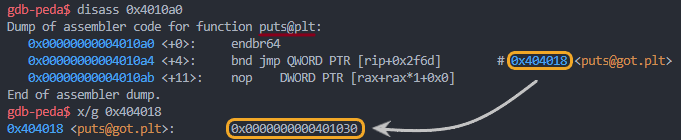
\includegraphics[width=0.70\textwidth]{images/puts-precall.png}
    \\
    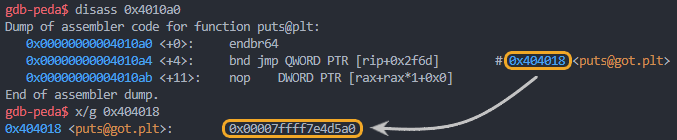
\includegraphics[width=0.70\textwidth]{images/puts-aftercall.png}
    \caption{\label{fig:plt}Esempio preso dai test del contenuto di ``\textbf{.got.plt}'' associato alla funzione esterna \textbf{puts}, \textbf{prima} e \textbf{dopo} una sua prima chiamata dall'applicazione.}
\end{figure}

Al termine di tale processo, sarà necessario calcolare l'indirizzo di partenza della libreria in memoria, andando a sottrarre l'indirizzo statico (quello prima della allocazione effettiva nella memoria) di tale funzione presente nel file ELF della libreria, a quello ottenuto nel punto precedente \cite*{Return2plt}.\\
Una volta ottenuta tale informazione, basterà sottrarre l'indirizzo statico della funzione (o delle funzioni) che si vuole richiamare a quello di base del punto precedente ed inserire tale dato all'interno di una nuova \textbf{ROP chain}, così da deviando conseguentemente il normale flusso del programma.

\subsection*{Attacco sovrascrivendo la GOT table}
\label{subsec:Attack_3.2.2}
Nel precedente approccio, si è affrontata una tecnica che consentiva di recuperare l'indirizzo di base della libreria in memoria, tuttavia questo non rappresenta l'unico modo per bypassare una difesa come \textbf{ASLR} utilizzando la \textbf{Return Oriented Programming}.\\
Quando nella sezione \ref{subsec:PLT-GOT} sono state introdotte le due sezioni \textbf{Procedure Linkage Table} e \textbf{Global Offset Table} presenti all'interno del file \textbf{ELF}, è stato omesso un dettaglio cruciale per questa tecnica riguardo la \textbf{GOT}, ossia che, a differenza della \textbf{PLT}, essa \underline{non è di tipo \textit{read-only}}.
È quindi possibile scrivere all'interno di tale sezione, alterandone gli indirizzi contenuti in essa.\\
L'idea che ruota attorno a questa tipologia d'attacco è che, se l'attaccante riesce a calcolare l'offset tra gli indirizzi statici di due funzioni nel file \textbf{ELF} della stessa libreria, come possono essere \textbf{puts} e \textbf{system} nella \textbf{libc}, sarà sufficiente attendere che il processo effettui la chiamata ad una delle due funzioni, nel caso \textbf{puts}, per aggiornare il contenuto del puntatore associato alla sua voce in ``\textbf{.got.plt}'', ed andare poi a sommare l'offset
calcolato in precedenza a tale indirizzo contenuto \cite*{GOT-OVERWRITE}\cite*{GOT-OVERWRITE-MITIGATION}.\\
Il risultato finale sarà che ad una qualsiasi prossima chiamata di tale funzione, verrà invece invocata la seconda subroutine di cui l'utente malevolo ha calcolato l'offset con la prima precedentemente, quindi nel caso specifico \textbf{system}.\\
Questo dettaglio apparentemente piccolo della sezione \textbf{GOT}, fornisce quindi una soluzione ulteriore per effettuare i propri attacchi sfruttando sempre la \textbf{ROP}.

\subsection{Attacco non conoscendo la versione della libc collegata}
\label{subsec:Attack_3.3}
Nella \hyperref[subsec:Attack_3.2]{prima} situazione, l'attaccante disponeva del file \textbf{ELF} della libreria, e grazie a ciò conosceva gli offset degli indirizzi delle funzioni all'interno di essa. Tuttavia, effettuando attacchi \textbf{ROP} da remoto o comunque non essendo possibile recuperare in alcun modo (senza utilizzare un exploit) la versione corrispondente delle librerie collegate all'applicazione attaccata, diviene essenziale trovare un metodo efficace per farlo.\\
Come visto nei due attacchi precedenti, è di fondamentale importanza avere a disposizione l'\textbf{ELF} delle librerie perché l'utente possa utilizzare le funzioni al loro interno, soprattutto se in presenza di difese come \textbf{ASLR}.\\
Solitamente, qualsiasi programma in linguaggio C fa utilizzo di almeno una funzione della \textbf{libc}, venendo conseguentemente collegata dinamicamente con esso \cite*{Ret2libc-libcexpl}. In questi casi, l'attaccante può provare a recuperare la versione della ``\textbf{standard C library}'' con un approccio molto simile a quello usato nella sezione \ref{subsec:Attack_3.2.1}.\\
In questo caso, servirà ottenere due indirizzi effettivi in memoria di funzioni appartenenti alla libreria, stampandoli inserendo due chiamate alla funzione \textbf{puts} nella \textbf{ROP chain}. Grazie ad essi, sarà possibile ricercare la corretta versione della libreria in alcuni database online contenenti i simboli di moltissime versioni di \textbf{libc}, come il seguente: \label{libc-db}\href{https://libc.blukat.me/}{libc database}. \cite*{find-libc-version}\\
Questo è possibile nonostante la presenza di ASLR, perché l'indirizzo di base della libreria in memoria terminerà sempre con la sequenza ``\textbf{000}'' per una questione di allineamento delle regioni di memoria. \cite*{find-libc-version2}
\begin{figure}[ht]
    \centerline{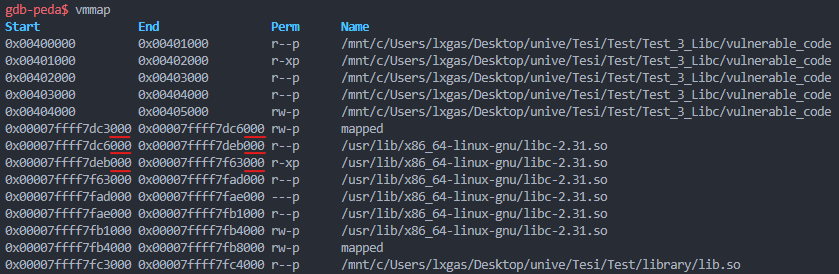
\includegraphics[scale=.5]{images/memory-paging.png}}
    \caption{Esempio di un possibile mapping di memoria, ogni indirizzo termina con la sequenza ``\textbf{000}''.}
    \label{fig:Mem-paging}
\end{figure}

Quindi ogni simbolo o indirizzo statico di \textbf{libc} terminerà sempre con la stessa sequenza di tre caratteri finali, nonostante la presenza di \textbf{ASLR}. Conseguentemente, gli offset tra i simboli saranno costanti per una particolare versione di essa.\\ 
Questi offset, recuperati dagli indirizzi ottenuti con la \textbf{ROP chain}, potranno essere allora cercati online nei \hyperref[libc-db]{database sopraccitati}.\\
Un esempio pratico può essere il seguente preso dai test effettuati, dove gli indirizzi ottenuti durante l'esecuzione dell'applicazione erano i seguenti: 
\begin{itemize}
    \item \textbf{puts} \space: \texttt{0x7f79ab24e5a0}
    \item \textbf{scanf}: \texttt{0x7f79ab22d230}
\end{itemize}
Nel primo caso l'offset sarà ``\textbf{\texttt{5a0}}'', mentre nel secondo sarà ``\textbf{\texttt{230}}''. Inserendoli nel database online si otterranno tre versioni della stessa libreria che non presenteranno particolari differenze l'una dall'altra. 

\begin{figure}[htbp]
    \centerline{\frame{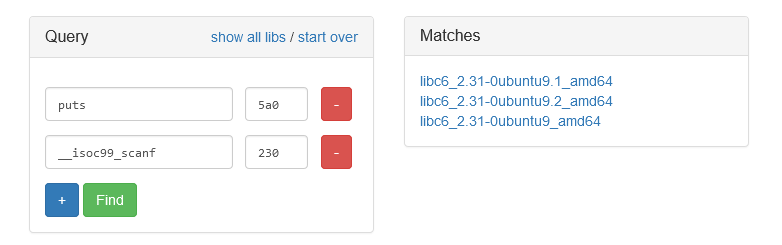
\includegraphics[scale=.45]{images/libc-database.png}}}
    \caption{Esempio di ricerca in uno dei database delle \textbf{libc}, inserendo due offset ottenuti dagli indirizzi in memoria delle funzioni \textbf{puts} e \textbf{scanf}.}
    \label{fig:libc-db}
\end{figure}

Recuperata la versione di \textbf{libc} corretta e calcolato l'indirizzo di base in memoria di essa come nell'attacco della sezione \ref{subsec:Attack_3.2}, l'attaccante potrà utilizzare qualsiasi funzione all'interno di essa grazie alla \textbf{Return Oriented Programming}, come ad esempio quella per eseguire una \textit{shell} \cite*{find-libc-version}.

\section{Attacco utilizzando la funzione \_\_libc\_csu\_init()}
\label{sec:Attack_4}
Accade spesso che in attacchi con protagonista la \textbf{Return Oriented Programming}, prima di inserire la chiamata di una determinata funzione all'interno della propria \textbf{ROP chain}, debbano essere prima impostati correttamente i contenuti di alcuni registri, nello specifico quelli previsti dalle \hyperref[call-convention]{convenzioni di chiamata utilizzata nell'architettura \textbf{x86-64}}, 
quindi \textbf{rdi}, \textbf{rsi}, \textbf{rdx}, \textbf{rcx}, \textbf{r8}, \textbf{r9}.\\
È molto comune infatti che le funzioni richiedano dai due ai tre parametri se non di più, per essere richiamate in maniera corretta. Per questo diviene spesso fondamentale poter controllare alcuni dei registri sopraccitati.\\
Il problema che si ci può ritrovare ad affrontare, nel caso di piccoli codici come quello visto nei test, è la mancanza di gadgets per controllare il contenuto di questi specifici registri.\\
A tale scopo, col passare degli anni è stata trovata una soluzione che per le sue potenzialità prese addirittura il nome di ``\textbf{Universal ROP}'' \cite*{return-to-csu-challenge}.\\ 
Questa tecnica, più comunemente definita ``\textbf{return-to-csu}'', riguarda nello specifico i sistemi GNU/Linux e prende nome da una particolare funzione definita \textbf{\_\_libc\_csu\_init}(), trovabile tra i simboli di un qualsiasi file \textbf{ELF} di un programma.\\
Essa fa parte di quello che viene chiamato ``\textbf{attached code}'', ossia simboli addizionali presenti nell'\textbf{ELF} di un'applicazione, non facenti parte del codice sorgente prima della sua compilazione. \cite*{return-to-csu}\\
Senza entrare troppo nei dettagli di questo fenomeno \cite*{return-to-csu2}, quello che l'ha reso particolarmente interessante per la creazione degli exploit, è la presenza di un \textbf{gadget} trovabile all'interno di \textbf{\_\_libc\_csu\_init}() che consente di controllare alcuni registri di primaria importanza come \textbf{edi}, \textbf{rsi}, \textbf{rdx} ed altri quali \textbf{rbp}, \textbf{rbx}, \textbf{r12}, \textbf{r13}, \textbf{r14}, \textbf{r15}.\\

\begin{figure}[htbp]
    \centerline{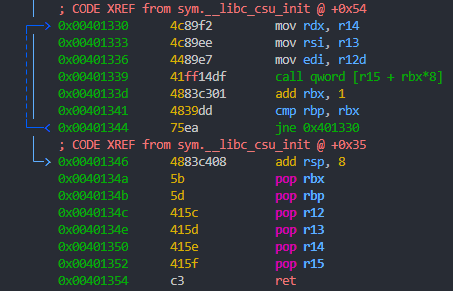
\includegraphics[scale=.65]{images/__libc_csu_init.png}}
    \caption{Gadget utilizzabile per controllare \textbf{edi}, \textbf{rsi}, \textbf{rdx}, \textbf{rbp}, \textbf{rbx}, \textbf{r12}, \textbf{r13}, \textbf{r14}, \textbf{r15}, disponibile per via di \textbf{\_\_libc\_csu\_init}().}
    \label{fig:csu-gadget}
\end{figure}

Come si vedrà successivamente nei test, questo \textbf{gadget} consente di gestire parecchi registri, tuttavia non senza un minimo di difficoltà. Infatti, nell'utilizzare tale sequenza è necessario fare attenzione ad un'istruzione in particolare (visibile anche in figura \ref{fig:csu-gadget}) che se non gestita in maniera corretta, può portare alla terminazione dell'applicazione:
\\\\\centerline{\texttt{\large{\textbf{\textcolor{Bittersweet}{call}  \space  qword [R15 + RBX*8];}}}}\\\\
Questa istruzione caricherà l'indirizzo di ritorno nello stack ed andrà ad eseguire quanto contenuto nell'indirizzo tra le due parentesi quadre.\\
Per far sì che l'esecuzione non termini, sarà necessario quindi passare a tale istruzione un puntatore ad un gadget, cosicché una volta terminata la subroutine in esso contenuta, verrà recuperato l'indirizzo di ritorno nello stack, e ripresa l'esecuzione dall'istruzione successiva alla ``\textbf{call}''.\\
Una volta trovato un opportuno puntatore, sarà sufficiente caricare il suo indirizzo nel registro \textbf{r15} ed azzerare invece il contenuto di \textbf{rbx}, per ottenere il risultato desiderato \cite*{return-to-csu2}.\\
Se usata con accortezza questa tecnica consentirà di gestire alcuni dei più importanti registri utilizzando la \textbf{Return Oriented Programming}, seppur avendo pochi \textbf{gadgets} a disposizione.

\section{Attacco con bypass dello ``stack canary''}
\label{sec:Attack_5}
Come ultimo attacco verrà affrontato quello che probabilmente rappresenta uno dei metodi più antichi utilizzati per rilevare alcune vulnerabilità all'interno dei codici, ossia quelli che vengono definiti ``\textbf{Stack Canaries}''.\\
Prima di entrare nel vivo dell'attacco verrà fatta un'introduzione a questa storica tecnica di difesa.

\subsection*{Gli ``stack canaries''}
\label{sec:stack canaries}
Gli \textbf{stack canaries} sono una delle più conosciute mitigazioni ad exploit che sfruttano gli \textbf{stack-based buffer overflow}.\\L'idea di base è quella di inserire un valore casuale chiamato appunto ``\textbf{canary}'' esattamente tra le variabili locali e i dati critici (come l'indirizzo di ritorno), in ogni stack frame generato \cite*{Canary}. Se l'attaccante proverà a sfruttare qualche vulnerabilità per sovrascrivere tali dati, sarà costretto a modificare pure questo speciale valore, visto il suo posizionamento
nello stack. Qualsiasi modifica apportata al ``\textbf{canary}'' sarà identificata durante il flusso di esecuzione dell'applicazione, più nello specifico subito prima di un'istruzione \textbf{ret} alla fine di una subroutine, con la conseguente terminazione di esso \cite*{Canary2}. 

\begin{figure}[htbp]
    \centerline{\frame{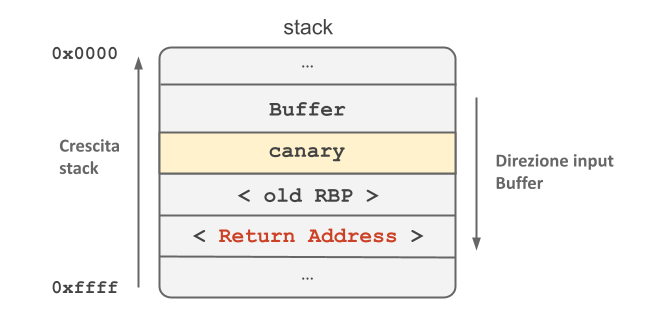
\includegraphics[scale=.4]{images/Canary.png}}}
    \caption{Esempio di stack contenente il ``\textbf{canary}''.}
    \label{fig:canary}
\end{figure}
Un utente non avrà quindi modo di ottenere il controllo del flusso del programma, visto che questa verifica di integrità sarà sempre effettuata prima di una qualsiasi istruzione \textbf{ret}.\\
Esistono diverse tipologie di \textbf{stack canaries}, ognuna in grado di offrire protezioni in modi differenti: 
\begin{itemize}
    \item \textbf{Terminator canary} \\
    Consiste di vari caratteri ed almeno uno di quelli definiti ``\textbf{terminatore di stringa}''\footnote[1]{I ``\textbf{caratteri terminatori di stringa}'' in linguaggio C sono speciali caratteri che hanno la funzione di delimitare la fine di una stringa.} (come \textit{new line}, \textit{null}, \textit{e.t.c.}).\\
    l'idea in questo caso è che siccome molte delle vulnerabilità nei codici sono dovute a funzioni quali \textbf{gets()}, \textbf{strcpy()}, l'attaccante non potrà inserire tali valori nel proprio input. Se per esempio si considera un overflow causato da una \textbf{gets()}, se il ``\textbf{canary}'' conterrà il carattere speciale \textit{new line} non potrà essere replicato dall'utente malevolo, in quanto tale funzione terminerà la lettura dell'input alla ricezione di quel carattere.
    \item \textbf{Random canary} \\
    Consiste di una sequenza random di byte sconosciuta all'attaccante. In questo caso, tale dato potrà essere replicato dall'utente se all'interno del codice sarà presente ad esempio una vulnerabilità di tipo \hyperref[subsec:format string]{\textbf{format string}}, che gli consenta quindi di recuperare tale valore dallo stack.
    \item \textbf{Random XOR canary} \\
    Come il \textbf{Random canary}, consiste di una sequenza random di byte a cui è stata effettuata una \textbf{XOR} utilizzando i dati di controllo nello stack (come \textbf{indirizzo di ritorno} oppure il precedente valore del registro \textbf{rbp}), aggiungendo un livello ulteriore di casualità. In questo caso, anche una modifica a tali dati porterà quindi ad alterare indirettamente il \textbf{canary}.\\
\end{itemize}
Nei primi due casi, risulterà comunque un sistema di difesa inutile se, come si vedrà nei test, l'attaccante potrà sovrascrivere indirizzi di memoria arbitrari, tramite delle vulnerabilità all'interno del codice, consentendogli di modificare i dati di controllo all'interno dello stack, come l'\textbf{indirizzo di ritorno}, senza alterare il canary.\\
Il terzo caso, invece, cerca di evitare attacchi come quello appena descritto mettendo assieme \textbf{random canary} e \textbf{dati di controllo}, bloccando l'esecuzione sia in caso di modifica del primo che del secondo. Tuttavia, se l'utente avrà comunque modo di recuperare tramite altre vulnerabilità i dati in memoria (\hyperref[subsec:format string]{\textbf{format string}}), il canary fallirà nuovamente nel suo obbiettivo.\\
A volte è anche possibile trovare le tre casistiche combinate assieme, quindi per fare un esempio, \textbf{random canary} con un \textbf{carattere terminatore di stringa} fisso al suo interno. Sono anche queste soluzioni adottabili, però in certi casi possono rendere il canary più semplice da indovinare avendo una casualità ridotta.\\
\begin{figure}[ht]
    \centerline{\frame{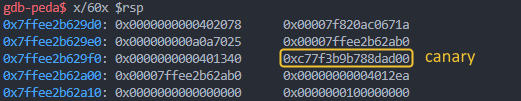
\includegraphics[scale=.5]{images/canary-stack.png}}}
    \caption{Esempio di stack canary in Linux, è tipico di questo sistema mettere un carattere di fine stringa come primo carattere del canary (ultimo nell'immagine per la notazione little indian).}
    \label{fig:canary-stack}
\end{figure}
In conclusione, gli \textbf{stack canaries} non sono sicuramente una difesa insuperabile, soprattutto in presenza di vulnerabilità che consentano di recuperare i dati in memoria. Questo non è sorprendente dal momento che furono creati per evitare l'exploit di vulnerabilità quali \textbf{buffer overflows}, e più nello specifico quelli inerenti allo stack. \cite*{Canary}

\subsection*{Bypass del canary}
\label{sec:canary bypass}
Come anticipato precedentemente, il canary all'interno dello stack può essere bypassato in presenza di diverse vulnerabilità ed in diversi modi, uno dei più classici è scoprendo il suo valore. L'opzione più semplice in questi casi è sfruttando le \hyperref[subsec:format string]{\textbf{format string}} se presenti all'interno del codice, altrimenti un'altra opzione può essere facendo quello che viene definito ``\textbf{bruteforce}'' dello stesso. Questa tecnica consiste nel testare tutti i
possibili caratteri uno dopo l'altro, avanzando di posizione fino a completamento ogni qualvolta ne sia stato trovato uno di corretto. Questo è possibile perché il canary viene generato ogni volta che l'applicazione viene eseguita, tuttavia, se vengono effettuate tante \textbf{fork}\footnote[1]{\textbf{fork()} è una funzione in Unix che porta a creare un secondo processo, detto \textbf{processo figlio}, identico al primo anche detto \textbf{processo padre}.} dello stesso processo, verrà mantenuto 
lo stesso canary anche nei processi figli, consentendo all'attaccante di effettuare un ``\textbf{bruteforce}'' su di esso. \cite*{Canary-bypass-brute}\\
Esistono altre tecniche per bypassare il canary, una di queste sarà quella utilizzata nel test \ref{sec:Test_5}. Tale tecnica prevede la sovrascrittura dell'indirizzo di un puntatore, su cui nelle fasi successive dell'esecuzione del programma, sarà possibile andare a scrivere. Se l'attaccante riuscirà a sostituire l'indirizzo del puntatore con quello dello stack su cui invece risiede l'indirizzo di ritorno, potrà utilizzare la \textbf{Return Oriented Programming} inserendo la propria 
\textbf{ROP chain} a partire da tale indirizzo, evitando conseguentemente di modificare il canary ed alterando comunque il flusso del programma.\\
In tale attacco si utilizzerà una vulnerabilità di tipo \hyperref[subsec:format string]{\textbf{format string}}, per recuperare l'indirizzo dello stack su cui risiede l'indirizzo di ritorno (\textbf{rbp}+8). Tale valore sarà poi sostituito grazie ad un \textbf{buffer overflow} a quello di un puntatore, su cui nelle fasi successive del programma sarà possibile scrivere. Una volta raggiunto tale punto, al posto del puntatore ci sarà l'indirizzo posto dall'attaccante e sarà quindi possibile andare a scrivere
direttamente sopra all'indirizzo di ritorno la \textbf{ROP chain}.
\\
Ora che sono state enunciate le idee su cui si basano queste differenti tecniche, con cui può essere applicata la \textbf{ROP}, verrà fatto un piccolo riepilogo riguardo le possibili mitigazioni a tali tecniche, ed in maniera generale alla \textbf{Return Oriented Programming}.

\section{Mitigation alla Return Oriented Programming}
\label{sec:mitigation}
Di seguito verranno brevemente introdotte alcune delle possibili mitigazioni contro gli attacchi \textbf{Return Oriented Programming} che sfruttano alcune delle vulnerabilità riguardanti la memoria.\\
\textbf{ProPolice} \cite*{Pro-Police} Oppure \textbf{Stack-Guard} \cite*{Stackguard} sono solo alcune delle tecniche in grado di prevenire i tradizionali attacchi basati sulla compromissione dello stack. Entrambi questi metodi sono buoni nella prevenzione dei tipici attacchi che sfruttano i \textbf{bufer overflow}, tuttavia sono noti alcuni metodi di elusione \cite*{StackGuard-bypass}, in grado di vanificarne parzialmente l'efficacia. \textbf{Bounds Checking} \cite*{BoundsChecking} è un'altra discreta tecnica che previene la corruzione 
delle aree di memoria alla radice, evitando lo sfruttamento da parte dell'attaccante di possibili overflow dei buffer.\\
Una delle meccaniche più efficaci in grado di assicurare il corretto flusso di esecuzione di un'applicazione è ``\textbf{Shadow Stack}''. Il concetto utilizzato in tale caso è quello di avere una specifica area di memoria dedicata esclusivamente all'archiviazione delle copie di backup di tutti gli indirizzi di ritorno. Al termine di una funzione, l'indirizzo di ritorno memorizzato nello stack frame attuale viene confrontato con quello in cima allo \textit{shadow stack} (l'esito sarà positivo solamente se il contenuto dello stack
non è stato alterato). Utilizzando questa tecnica si può sconfiggere gli attacchi \textbf{Return Oriented Programming}, in quanto l'utente dovrebbe sovrascrivere sia l'indirizzo di ritorno memorizzato nello stack che quello archiviato nello \textit{shadow stack}. L'unico problema che persiste con questa tecnica è che protegge solamente tale indirizzo, non fornendo quindi una protezione verso attacchi di tipo \hyperref[jop]{\textbf{JOP}}. A tale scopo \textbf{Intel} ha introdotto e successivamente rilasciato la 
\textbf{Control-flow Enforcement Technology} (\textbf{CET}), una funzionalità all'interno dei nuovi processori che sfrutta anche il concetto dello \textit{shadow stack} per prevenire sia attacchi \textbf{ROP} che \textbf{JOP} \cite{CET}.\\
Infine, i sistemi di protezione del flusso di controllo (\textbf{Control-flow integritiy} o \textbf{CFI}) \cite*{CFI1}\cite*{CFI2} possono impedire che il controllo del flusso di un programma venga dirottato. Alcune implementazioni di tali sistemi prevedono l'esclusiva esecuzione delle istruzioni necessarie per il normale flusso del programma, escludendo conseguentemente molti dei \textbf{gadgets} che potrebbero essere invece utilizzati.\\
Dopo aver riassunto quelle che sono le principali meccaniche di difesa dagli attacchi \textbf{Return Oriented Programming}, nel prossimo capitolo verranno illustrati i test che sono stati effettuati utilizzandola ed applicando le tecniche viste in precedenza.
